\documentclass[11pt]{article}
\usepackage[utf8]{inputenc}
\usepackage{graphicx}
\usepackage{caption}
\usepackage{circuitikz}
\usepackage{geometry}
\geometry{letterpaper, margin=1in}

\title{PHYS 338K Final Project Proposal: Op-Amp Based Function Generator}
\author{Anna Grove and Lily Nguyen \\ Phys.338K}
\date{October 29, 2024}

\begin{document}

\maketitle

\section*{1. Project Description}

This project will design and build a function generator capable of producing sine, square, and triangle waves. In response to feedback, the design will not use a dedicated waveform generator IC (e.g., ICL8038). Instead, it will be constructed from discrete op-amps to provide a more challenging and educational experience.

The core of the generator will be a two-op-amp oscillator that produces simultaneous square and triangle waves with amplitudes that remain constant when the frequency is tuned. This addresses a key limitation of simpler integrator-based designs. The triangle wave output will then be fed into a diode-based nonlinear waveshaping circuit to generate a low-distortion sine wave approximation. The final outputs will be buffered to provide a low-impedance source.

\section*{2. Circuit Diagram}

\subsection*{Block Diagram:}
\begin{center}
    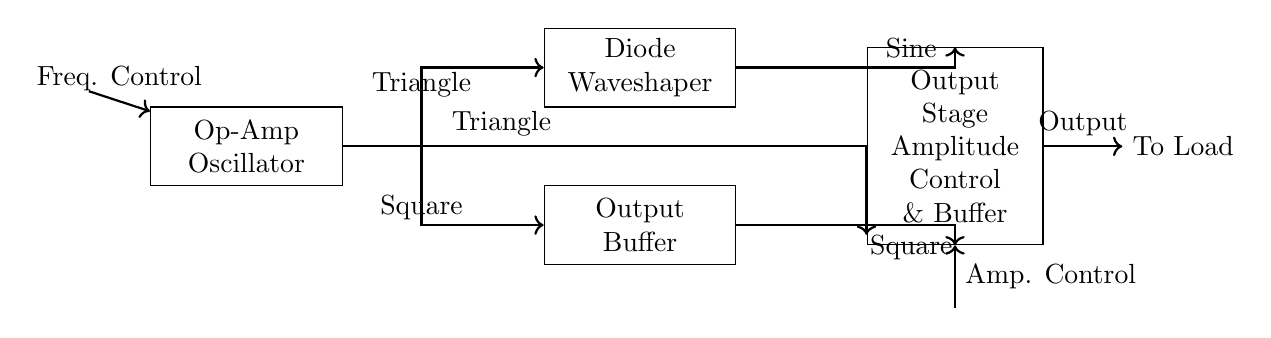
\begin{tikzpicture}
        % Nodes
        \draw (0,0)     node[draw, text width=2.2cm, align=center, minimum height=1cm] (osc) {Op-Amp\\Oscillator};
        \draw (5,1)     node[draw, text width=2.2cm, align=center, minimum height=1cm] (shape) {Diode\\Waveshaper};
        \draw (5,-1)    node[draw, text width=2.2cm, align=center, minimum height=1cm] (bufB) {Output\\Buffer};
        \draw (9,0)     node[draw, text width=2cm, align=center, minimum height=2.5cm] (mux) {Output Stage\\Amplitude Control\\\& Buffer};
        
        % Oscillator Outputs
        \draw[->, thick] (osc.east) -- ++(1,0) |- (shape.west) node[pos=0.25, above] {Triangle};
        \draw[->, thick] (osc.east) -- ++(1,0) |- (bufB.west) node[pos=0.25, below] {Square};
        
        % Paths to Output Stage
        \draw[->, thick] (shape.east) -| (mux.north) node[pos=0.4, above] {Sine};
        \draw[->, thick] (bufB.east) -| (mux.south) node[pos=0.4, below] {Square};
        \draw[->, thick] (osc.east) -- ++(1.5,0) -- ++(0,0) -| (mux.-135) node[pos=0.05, above] {Triangle}; % Direct path
        
        % Control Inputs
        \draw[->, thick] (-2, 0.7) -- (osc.160) node[midway, above] {Freq. Control};
        \draw[->, thick] (mux.south) ++ (0,-0.8) -- (mux.south) node[midway, right] {Amp. Control};
        
        % Final Output
        \draw[->, thick] (mux.east) -- ++(1,0) node[above, midway] {Output} node[right] {To Load};
    \end{tikzpicture}
\end{center}

\subsection*{Detailed Schematic:}

\textbf{Part (a): Two Op-Amp Triangle/Square Wave Oscillator (Constant Amplitude)}
\begin{center}
\begin{circuitikz}[scale=0.9]
    % Op-Amps
    \node[op amp, label={[font=\footnotesize]above:U1}] (opamp1) at (0,0) {};
    \node[op amp, label={[font=\footnotesize]above:U2}] (opamp2) at (6,0) {};
    
    % U1 as Schmitt Trigger
    % Positive Feedback
    \draw (opamp1.+) to[short] ++(0,-1) coordinate (feedbackDiv);
    \draw (feedbackDiv) to[R, l=$R_3$, a=4k$\Omega$] ++(0,-2) node[ground](gnd1){};
    \draw (opamp1.out) to[short, *-] ++(0,1) -| (feedbackDiv -| opamp1.+) to[short] (feedbackDiv -| opamp1.+);
    \draw (opamp1.out) to[short, *-] (opamp1.out -| opamp2.+) to[R, l=$R_2$, a=2k$\Omega$] (opamp2.+);
    
    % U2 as Integrator
    \draw (opamp2.-) to[short] ++(0,1.5) coordinate (topC);
    \draw (topC) to[C, l=$C_1$, a=1$\mu$F] (topC -| opamp2.out) to[short] (opamp2.out);
    \draw (opamp2.-) to[short] ++(-1,0) to[R, l=$R_1$] ++(-2,0) coordinate (leftR1);
    \draw (opamp1.out) to[short] (opamp1.out) -- (leftR1 |- opamp1.out) to[short] (leftR1);
    
    % Outputs
    \draw (opamp1.out) to[short, -o] ++(1,0) node[right] {Square Wave Out};
    \draw (opamp2.out) to[short, -o] ++(1,0) node[right] {Triangle Wave Out};
    
    % Power (simplified)
    \draw (opamp1.up) to[short, -o] ++(0,0.3) node[above] {$+V_{CC}$};
    \draw (opamp1.down) to[short, -o] ++(0,-0.3) node[below] {$-V_{EE}$};
    \draw (opamp2.up) to[short] (opamp2.up |- opamp1.up) to[short] (opamp1.up);
    \draw (opamp2.down) to[short] (opamp2.down |- opamp1.down) to[short] (opamp1.down);
    
    % Frequency Control Note
    \node[align=left, text width=6cm, font=\scriptsize, anchor=west] at (0, -4) {\textbf{Note:} Frequency is tuned by varying $R_2$ (potentiometer). The amplitudes of the square and triangle waves remain constant.};
\end{circuitikz}
\end{center}

\textbf{Part (b): Diode-Based Triangle-to-Sine Wave Shaper}
\begin{center}
\begin{circuitikz}[scale=0.85]
    % Input
    \draw (0,0) node[left] {Triangle Wave In} to[short, o-] (0.5,0);
    
    % Input resistor
    \draw (0.5,0) to[R, l=$R_{11}$, a=10k$\Omega$] (2.5,0);
    
    % Diode-resistor network
    \draw (2.5,0) -- (3,0);
    
    % Top half of the network (positive clipping)
    \draw (3,0) -- (3,1) to[R, l=$R_1$] (5,1) to[D*, l=$D_1$] (7,1) -- (7,0.3);
    \draw (3,0) -- (3,1.5) to[R, l=$R_2$] (5.5,1.5) to[D*, l=$D_2$] (7,1.5) -- (7,0.6);
    \draw (3,0) -- (3,2) to[R, l=$R_3$] (6,2) to[D*, l=$D_3$] (7,2) -- (7,0.9);
    \draw (3,0) -- (3,2.5) to[R, l=$R_4$] (6.5,2.5) to[D*, l=$D_4$] (7,2.5) -- (7,1.2);
    
    % Bottom half of the network (negative clipping)
    \draw (3,0) -- (3,-1) to[R, l=$R_5$] (5,-1) to[D*, l=$D_5$, invert] (7,-1) -- (7,-0.3);
    \draw (3,0) -- (3,-1.5) to[R, l=$R_6$] (5.5,-1.5) to[D*, l=$D_6$, invert] (7,-1.5) -- (7,-0.6);
    \draw (3,0) -- (3,-2) to[R, l=$R_7$] (6,-2) to[D*, l=$D_7$, invert] (7,-2) -- (7,-0.9);
    \draw (3,0) -- (3,-2.5) to[R, l=$R_8$] (6.5,-2.5) to[D*, l=$D_8$, invert] (7,-2.5) -- (7,-1.2);
    
    % Summing point and output amplifier
    \draw (7,0) -- (8,0) node[op amp, anchor=+, noinv input up] (opamp) {};
    \draw (opamp.-) -- ++(0,1.5) to[R, l=$R_f$] ++(2.5,0) -| (opamp.out) to[short, -*] (opamp.out);
    \draw (opamp.out) to[short, -o] ++(1,0) node[right] {Sine Wave Out};
    
    % Power for op-amp
    \draw (opamp.up) to[short, -o] ++(0,0.3) node[above] {$+V_{CC}$};
    \draw (opamp.down) to[short, -o] ++(0,-0.3) node[below] {$-V_{EE}$};
    
    % Network output resistor
    \draw (7,0) to[R, l=$R_9$, a=2k$\Omega$] (opamp.+);
    \draw (opamp.+) to[short] ++(0,-1) node[ground]{};
    
    % Note
    \node[align=left, text width=10cm, font=\scriptsize, anchor=north] at (5, -4) {\textbf{Circuit (b) Description:} This network uses biased diodes ($D_1$-$D_8$) to progressively clip the peaks of the triangle wave, rounding it into a sine wave. Resistors $R_1$-$R_8$ set the bias points for the diodes. The op-amp sums the currents from the network.};
\end{circuitikz}
\end{center}

\section*{3. Revised Parts List}
\begin{itemize}
    \item \textbf{Op-Amps:} 3-4 x LM741, TL081, or similar general-purpose op-amps
    \item \textbf{Diodes:} 8 x 1N4148 or 1N914 small-signal switching diodes
    \item \textbf{Resistors:} Multiple values for oscillator, waveshaper, and biasing (e.g., 1k$\Omega$, 2k$\Omega$, 4k$\Omega$, 6.8k$\Omega$, 10k$\Omega$)
    \item \textbf{Capacitors:} 1$\mu$F timing capacitor and decoupling capacitors
    \item \textbf{Potentiometers:} One for frequency control ($R_2$), one for output amplitude control
    \item \textbf{Switch:} Single Pole, 3-Position (SP3T) rotary switch for waveform selection
    \item \textbf{Power Supply:} $\pm$9V or $\pm$12V dual rail supply
    \item \textbf{Output Connector:} BNC or 3.5mm audio jack
    \item \textbf{Breadboard/PCB:} For prototyping and final assembly
\end{itemize}

\end{document}